%
% Copyright (C) 2001 by Holger Karl,
% karl@ft.ee.tu-berlin.de
%
% file: template.tex
%
% Time-stamp: Sat Oct 06 08:29:52 2001
%
% Template fuer die Ausarbeitungen zu TKN-Seminaren
%
\documentclass[12pt,twoside,doublepage]{article}
\usepackage{url}
\def\UrlBreaks{\do\/\do-}

% Hier den Namen des Teilnehmers und den Titel  der Ausarbeitung eintragen:
\newcommand{\teilnehmer}{Abdul Ahad Ayaz}
\newcommand{\ausarbeitung}{AINFV: Analysis of Isolation (memory/packet) in Network Function Virtualization \newline Overview}
%AINFS
%Replace current memory/packet isolation techniques (e.g. Containers/VMs) used by
%Network Functions with Software Isolation

% Falls die Ausarbeitung in Deutsch erfolgt,
% die folgenden Kommentar-Zeichen '%' entfernen, andernfalls diese
 % Kommandos auskommentiert lassen:
% Languages:
% \usepackage[german]{babel}
% \usepackage[T1]{fontenc}
% \usepackage[latin1]{inputenc}
% \selectlanguage{german}

%%%%%%%%%%%%%%%%%%%%%%%%%%%
% Im restlichen Vorspann KEINE Aenderungen machen!
%%%%%%%%%%%%%%%%%%%%%%%%%%%
\usepackage{times}
\usepackage{url}

\usepackage[numbers]{natbib}

\usepackage{geometry}
\geometry{a4paper,body={5.8in,9in}}

% Graphics:
\usepackage{graphicx}
% aller Bilder werden im Unterverzeichnis figures gesucht:
\graphicspath{{figures/}}

% Headers:
\usepackage{fancyhdr}
% \pagestyle{fancy}
\pagestyle{fancy}
\fancyhead{}
\fancyhead[LE]{ \slshape \teilnehmer}
\fancyhead[LO]{}
\fancyhead[RE]{}
\fancyhead[RO]{ \slshape \ausarbeitung}
\fancyfoot[C]{}

\begin{document}

\title{\ausarbeitung}
\author{\teilnehmer}
\date{}
\maketitle
\thispagestyle{empty}

%%%%%%%%%%%%%%%%%%%%%%%%%%%%%%%%%%%%%%
% ab hier steht der eigentliche Text:


% Abstract gives a brief summary of the main points of a paper:
%\begin{abstract}
 % This paper gives a brief overview of the use of pigeon as a physical
 % layer underlying  the IP protocol. 
%\end{abstract} 

% the actual content, usually separated over a number of sections
% each section is assigned a label, in order to be able to put a
% crossreference to it

\section*{Summary}
%\label{sec:introduction}
Network Function Virtualization (NFV) is a new way of defining network with the help of software that way previously done with hardware middle-boxes. These days, Service Providers fully utilize the IT Virtualization Technologies (using commodity servers) for fast deployment of new network services with minimal cost. In 2012, ETSI\cite{ETSI2012} was formed that defined the requirements and standardization of NFV. There is performance overhead between NFV and hardware middle-boxes in terms of packet transfer rate, latency etc. Another main thing to consider is the isolation, there are two types: memory isolation and packet isolation. Memory isolation is memory used by one NF should not be accessible by another NF, this can be done by using VMs/Containers. Packet isolation is when NFs are chained, at any point in time only one NF should have the reference to that particular packet. Packet isolation is hard to achieve as compared to memory isolation in NFV as it involve the copying of the packets from one NF to other using vSwitch. These isolations ensures security but at the cost of performance. The performance metric used are packet processing (i.e. Million Packets per Second [MPPS]) and latency. The model paper NetBricks\cite{Panda2016} framework ensure the above isolations without the use of multiple VMs/Containers and packet copying using vSwitch. All NFs are chained in a single VM and communicate using function call. It provides the same performance as without using any isolation. NetBricks provide the high-level abstractions using RUST\cite{TheRustTeam2016} to developers for new developments and low-level optimization. Prior to NetBricks many advancements had been done to ensure the isolation, but the performance was not up to the mark for example: NetVM\cite{Hwang2015}, xOMB\cite{Anderson2012}, ClickOS\cite{Martins2014}, mSwitch\cite{Honda2015}, HyperSwitch\cite{Ram2013}. NetVM is virtualization-based platform. It has shared memory that uses DPDK\cite{Corporation2014} for zero-copy delivery between VMs ensuring isolation. ClickOS uses the Click\cite{Kohler2000} as a main programming model for middle-boxes and creating minimal OS . It runs in para-virtualized environment. It ensures the isolation and low packet delay. HyperSwitch is virtualization-based platform, it implements the virtual switch inside the hypervisor for inter-VMs communication and ensure memory isolation. Most of the above mentioned developments used VMs/Containers i.e one NF per VM/Container for isolation. OpenNetVM\cite{Yurchenko2018} framework is similar to NetBricks and is based on NetVM architecture using Dockers Container. SafeBricks\cite{Poddar2018} is based on NetBricks framework. It is used to protect the traffic processing in cloud by executing the NFs in \textit{hardware enclaves}(i.e. Intel SGX\cite{McKeen2013}). HyperNF\cite{Yasukata2017} framework is used to fully utilized the available resources(i.e. CPU cores) for processing. Packet processing is done using the hypercall instead of involving the vSwitch every time. HyperNF is based on standard NFV architecture whereas NetBricks  rewrites the software middle-boxes. libVNF\cite{Naik2017} is an open-source library that provide the high-level abstractions as NetBricks. It also enables clustered VNF implementations that are not supported by the NetBricks. YANFF\cite{Philippov2017} framework provides high-level abstraction using Go language. It uses the scheduler for packet processing over multiple cores, whereas in NetBricks it is done by shuffle calls. G-NET\cite{Zhang2018} is based on GPU virtualization, GPU scheduler is used to optimize the throughput. G-NET uses \textit{IsoPointer} for data isolation.
\nocite{*}

%The introduction describes the problem, why it is important, the main
%ideas of the following paper, what are the main contributions of the
%paper, etc. 

%\section{Related Work}
%\label{sec:relwork}

%The related work section could describe other work that is in some
%respects relevant for the understanding of the problem outlined in
%Section~\ref{sec:introduction}, that offer competing solutions, etc.

%All sources must be properly referenced, ideally by using the BiBTeX
%system. References can then be very conveniently made with the
%\texttt{cite} command. For example, reference
%\citenum{leuwen00:_handb_schol} discusses some of the elementary rules on
%writing scientific papers, amongst others how to correctly cite other
%documents. \citeauthor{Taylor:SIGuide:95}, e.g., describes how to
%correctly use the SI system of units and their correct typographical
%representation \citep{Taylor:SIGuide:95}. 

%Since we are using the  \texttt{natbib} package in this template, it is also convenient to
%to directly refer to the author names via the cite command -- see
%above for an example and check the natbib manual,\footnote{\url{http://www.ctan.org/tex-archive/macros/latex/contrib/natbib}}  very powerful!



%\section{Model description}
%\label{sec:model}

%After the two common sections Introduction and Related work, more
%sections with the actual content of a paper follow. The style and
%structure of such sections varies by a large degree, no general rules
%of thumb can be given. 

%Such a section could, among other things, include a figure. Note that
%a figure is a so-called floating object: it is moved around the actual
%text in order to best fit on a page. This is in stark contrast to some
%GUI-based word processing tools, where the placement of figures is
%usually more associated with luck than principle.

%As figures float around, expressions like ``the following figure''
%must never be used. Instead, figures need a caption, a label, and must
%be properly referenced in the main text. An example for this concept
%is shown in Figure~\ref{fig:example}. 

%\begin{figure}[htbp]
%  \begin{center}
 %   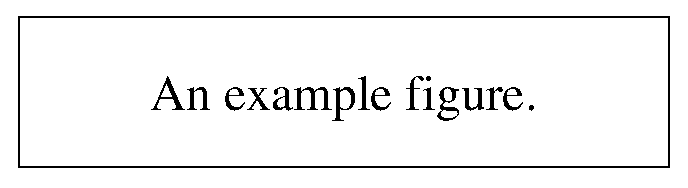
\includegraphics{example}
  %  \caption{An example figure with a caption.}
   % \label{fig:example}
%  \end{center}
%\end{figure}

%In general, only vector graphics in encapsulated postscript (eps)
%format should be included in any kind of text, as this allows arbirary
%scaling, rotation etc.\ without any loss of quality. Bitmap formats
%(JPEG, GIF, \dots) should only be used if no other alternative exists
%--- basically the only case where bitmaps can be justified is when
%scanned pictures need to be included in a text, however, this should
%be avoided as hard as possible as the quality in usually not
%satisfactory. EPS files can easily be produced by most tools; for
%particular difficult cases, tools like WMF2EPS can be helpful. 

%\section{Word processing \& \LaTeX}
%\label{sec:latex}

%This document has already introduced the most important constructs of
%\LaTeX. What is necessary to produce documents with \LaTeX is simple
%any normal text editor and a \LaTeX distribution. This is commonly
%installed on practically all UNIX-type systems; for Windows, an
%excellent \LaTeX exists, called MikTeX, available from
%\url{www.miktex.org}. Almost all distributions come with a large patch
%of examples and introductory material; consult your local installation
%for details. 

%Lots of supplementary and background information, FAQs, etc.\ is
%available from the Comprehensive TeX Archive Network (CTAN); the
%German mirror of which is \url{www.dante.de}. 

%\section{Conclusion}
%\label{sec:concl}

%At the end, there is a final section concluding and summarizing a
%paper, putting the entire work into perspective and explaining, on a
%larger level, what the consequences of this work are. Also, unexpected
%results can be discussed here, etc.


%%%%%%%%%%%%%%%%%%%%%%%%%%%%%%%%%%%%%%
% give a pointer to the bibliography information: 
\bibliography{bib}

%%%%%%
% we use natbib
\bibliographystyle{plainnat}

\end{document}


